\documentclass[12pt]{standalone}
\usepackage{tikz}

\begin{document}
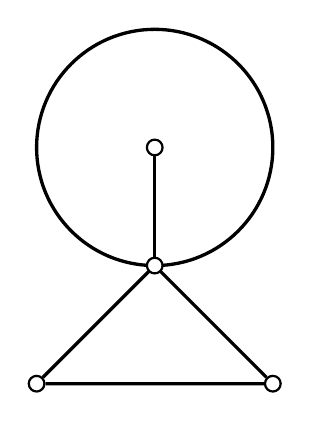
\begin{tikzpicture}[scale=1.5]
    \coordinate (a) at (0,0);
    \node[circle, thick, draw, inner sep=2pt] (b) at (0,1) {};
    \node[circle, thick, draw, inner sep=2pt] (c) at (-1,-1) {};
    \node[circle, thick, draw, inner sep=2pt] (d) at (+1,-1) {};
    \draw[very thick, black] (a) -- (b);
    \draw[very thick, black] (b) circle (1);
    \draw[very thick, black] (a) -- (c) -- (d) -- (a);
    \node[circle, thick, draw, fill=white, inner sep=2pt] at (a) {};
\end{tikzpicture}
\hspace{40pt}
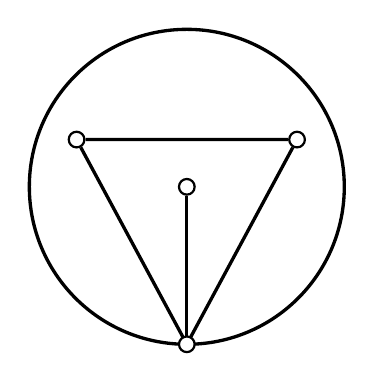
\begin{tikzpicture}[scale=2]
    \coordinate (a) at (0,0);
    \node[circle, thick, draw, inner sep=2pt] (b) at (0,1) {};
    \node[circle, thick, draw, inner sep=2pt] (c) at (-0.7,1.3) {};
    \node[circle, thick, draw, inner sep=2pt] (d) at (+0.7,1.3) {};
    \draw[very thick, black] (a) -- (b);
    \draw[very thick, black] (b) circle (1);
    \draw[very thick, black] (a) -- (c) -- (d) -- (a);
    \node[circle, thick, draw, fill=white, inner sep=2pt] at (a) {};
\end{tikzpicture}
\end{document}
